%--------------------
% Packages
% -------------------
\documentclass[11pt,a4paper]{article}
\usepackage[utf8x]{inputenc}
\usepackage[T1]{fontenc}
%\usepackage{gentium}
\usepackage{mathptmx} % Use Times Font

\usepackage[pdftex]{graphicx} % Required for including pictures
\usepackage[pdftex,linkcolor=black,pdfborder={0 0 0}]{hyperref} % Format links for pdf
\usepackage{calc} % To reset the counter in the document after title page
\usepackage{bbm}
\usepackage{amsfonts,amssymb,amsbsy,amsmath}
\usepackage{mathtools}
\usepackage[inline]{enumitem}
\usepackage{bm}



\frenchspacing % No double spacing between sentences
\linespread{1.2} % Set linespace
\usepackage[a4paper, lmargin=0.1666\paperwidth, rmargin=0.1666\paperwidth, tmargin=0.1111\paperheight, bmargin=0.1111\paperheight]{geometry} %margins
%\usepackage{parskip}

\usepackage[all]{nowidow} % Tries to remove widows
\usepackage[protrusion=true,expansion=true]{microtype} % Improves typography, load after font package is selected


\usepackage{lipsum} % Used for inserting dummy 'Lorem ipsum' text into the template

\newcommand{\tr}[1]{\texttt{Tr}\left\{ #1 \right\}}
\newcommand{\Pest}{P_{t+1|t}^{(k)}}
\newcommand{\etal}{\textit{et al}.~}
\newcommand{\Epolicy}[1]{\mathrm{E}_\pi \left[ #1 \right]}
\newcommand{\Ss}{\mathcal{S}}
\newcommand{\As}{\mathcal{A}}
\newcommand{\Rs}{\mathcal{R}_{ss'}^a}
\newcommand{\Pt}{\mathcal{P}_{ss'}^a}
\newcommand{\argmax}{\text{argmax}}
\newcommand{\egreedy}{$\epsilon$-greedy~}
\newcommand{\E}[1]{\mathrm{E}\left[ #1 \right]}
\newcommand{\inv}[1]{#1^{-1}}
\renewcommand{\Pr}[1]{\text{Pr}\left\{ #1 \right\}}

\newcommand{\xprior}{\hat{\vec{x}}_{k|k-1}}
\newcommand{\xpost}{\hat{\vec{x}}_{k|k}}
\newcommand{\xlast}{\hat{\vec{x}}_{k-1|k-1}}

\newcommand{\priorpcov}{\vec{P}_{k|k-1}}
\newcommand{\postpcov}{\vec{P}_{k}}
\newcommand{\lastpcov}{\vec{P}_{k-1|k-1}}

\newcommand{\prefitinnov}{\Tilde{\bm{y}}_k}
\newcommand{\postfitinnov}{\Tilde{\bm{y}}_{k|k}}

\renewcommand{\vec}[1]{\mathbf{#1}}
\renewcommand{\Vec}[1]{\boldsymbol{#1}}


\newcommand{\x}{\bm{x}_k}
\newcommand{\xnext}{\bm{x}_{k+1}}

\newcommand{\z}{\bm{z}_k}
\newcommand{\znext}{\bm{z}_{k+1}}

\newcommand{\stmodel}{\vec{F}_k}
\newcommand{\cimodel}{\vec{B}_k}
\newcommand{\cinput}{\vec{u}_k}
\newcommand{\pnoise}{\vec{w}_k}
\newcommand{\omodel}{\vec{H}_k}

\newcommand{\onoise}{\vec{v}_k}
\newcommand{\ocov}{\vec{R}_k}
\newcommand{\pcov}{\vec{Q}_k}
\newcommand{\innocov}{\vec{S}_k}

\newcommand{\eye}{\vec{I}}
\newcommand{\gain}{\vec{K}_k}

\newcommand{\normal}[2]{\mathrm{N}\left(#1, #2 \right)}


\DeclarePairedDelimiter\ceil{\lceil}{\rceil}
\DeclarePairedDelimiter\floor{\lfloor}{\rfloor}

\title{Reinforcement Learning Based Revisit Interval Selection for Multifunction Radars}
\author{\large Petteri Pulkkinen}


%-----------------------
% Set pdf information and add title, fill in the fields
%-----------------------
\hypersetup{ 	
pdfsubject = {},
pdftitle = {},
pdfauthor = {}
}

%-----------------------
% Begin document
%-----------------------
\begin{document} %All text i dokumentet hamnar mellan dessa taggar, allt ovanför är formatering av dokumentet

\maketitle
\tableofcontents

\newpage
\section{Introduction}

A modern air surveillance radar can carry out multiple different radar functions simultaneously.
Those functions include target tracking, target classification, and search for undetected targets.
Radars that can carry out multiple different functions are generally called multifunction radars.
The key technology that has enabled multiple functions to be performed concurrently is phased-array technology such as
electronically scanned arrays (AESA).
The phased array technology enables radars to electronically steer the electromagnetic energy to the desired direction with relatively low delay.

An important problem in multifunction radars is to determine how to share the limited time budget among the different tasks.
Consequently, phased-array technology creates a great opportunity to improve air surveillance radar performance by using more efficient time budget management (TBM) algorithms.
The performance of a TBM algorithm is typically dependent on the following quantities 
\begin{enumerate*}[label=(\roman*)]
    \item the number of tracks the radar is capable to handle,
    \item the tracking accuracy, and
    \item the probability of observing undetected targets in the surveillance volume.
\end{enumerate*}
An efficient TBM algorithm is needed to maximize the benefit of using phased-array technology.

Assigning the radar time resources for multiple tasks in multifunction radars have been intensively studied by the research community.
Different names have emerged for the problem such as resource management \cite{Wintenby2006, Charlish2015a} and scheduling \cite{Esfahani2012, Byrne2015, Byrne2016, Krishnamurthy1999, Krishnamurthy2001}.
In general, resource management is intended to denote controlling any of the radar resources such as energy budget, time budget, phase shifting budget, and processing budget \cite{Ding2008}.
Moreover, the scheduling can be interpreted as to be a low-level scheduling algorithm \cite{Wintenby2006}.
In this thesis, the term "time budget management" is used, because it does not assign any expectations on how the actual objective is achieved.

Reinforcement learning (RL) has gained a great interest in the research community during recent years.
Specifically, the deep learning techniques have enabled applying RL to application domains that were before unavailable.
A survey by Luong \etal reveals that many different tasks can be approached with deep reinforcement learning techniques in communications and networking applications \cite{Luong2018}.
Other research areas that have shown interest in RL are for example robotics \cite{Kober2013} and smart grids \cite{Zhang2018}.
On the other hand, 
RL for radar applications has not been researched as extensively as it has been researched in other domains.
However, Hayking in \cite{Haykin2006} assumed that RL based approaches would be a significant direction for cognitive radar technology.
Current research papers in RL for radars include 
jamming strategies \cite{Qiang2017, Wang2019, Wang2019a, Zhang2019},
anti-jamming strategies \cite{Kang2018, Ak2019}, 
bandwidth allocation in environments with interfering communications system \cite{Selvi2018, Kozy2019},
selecting transmit frequency to improve detection performance in environments with clutter \cite{Wabeke2010}, 
information theoretic time budget management for multitarget tracking \cite{Kreucher2005, Xu2010},
a low-level scheduling algorithm for multichannel multifunction radars \cite{Shaghaghi2018},
selecting number of angle cells to be included into beam pattern in colocated MIMO radar \cite{Wang2018}, 
and sequential operation mode selection to improve detection performance for moving radar platform \cite{Smits2008}.

In this thesis, a reinforcement learning approach is proposed to address the TBM problem.
Moreover, a reinforcement learning algorithm is applied to control the revisit interval of the tracking filter.
The intention is to release resources from target tracking to other radar functions when the target movement is more predictable.
The reinforcement learning approach is capable of learning directly from the experience such that the environment model is not needed to optimize the employed reward function.
For example, the algorithm could be applied for various different tracking filters with minimal modification on the actual reinforcement learning formulation.  
Moreover, RL methods can learn to utilize observation data with a non-trivial connection to the revisit interval.
It was shown in \cite{Charlish2015} that the POMDP framework can be utilized to introduce anticipation for controlling the revisit interval.
The reinforcement learning approach can include the anticipation for taking long-term consequences in account when planning the 
tracking revisit intervals.

The thesis is organized as follows. !!! Write here when the thesis is written !!!

\newpage
\section{Theory}
\subsection{Markov decision processes} \label{sec:MDP}

\begin{itemize}
    \item Emphasize the significance of Markov chain and Markov property
    \item Actions are used to modify the Markov chain state transition probabilities
    \item Figure could be viable desirable to illustrate states and actions
\end{itemize}

Markov decision process (MDP) is a significant mathematical framework that is used formalize reinforcement learning problems \cite{Sutton2018}.
Generally, MDPs are used to address sequential decision-making problems where state transitions and rewards are deterministic or stochastic.
All MDPs include an agent which sequentially interacts with an environment and receives rewards from a certain reward distribution.
The key element of MDP is that the environment is modeled with a Markov chain.
The Markov chain has states $s \in \Ss$ and transition probabilities $p_{ss'}$ between the states $s$ and $s' \in \Ss$.
Essential property of Markov chains that is called Markov property is  
\begin{equation} \label{eq:markov_property}
    \Pr(S_{t+1} | S_t, A_t) = \Pr(S_{t+1} | S_t, A_t, S_{t-1}, A_{t-1}, ..., S_1, A_1, S_0, A_0),
\end{equation}
which implies that the future states of the Markov chain depends only on the current state and the action.
It means that it is enough for the agent to act based on the current Markov chain state.

The interaction means that agent can affect the transition probabilities $p_{ss'}$.
Therefore, the transition probability matrix $P(a)$ is function of the action $a\in \As$ that the agent can decide.
The dynamics of MDP can be summarized with a single probability distribution
\begin{equation}\label{eq:MDP_probs}
    p(s', r | s, a) = \Pr \{ S_{t+1}=s', R_{t+1}=r | S_t=s, A_t=a \}.
\end{equation}
which is the probability that environment changes from state $s$ to state $s'$ and receives immediate reward $r$ when action $a$ is taken.

The objective of the agent is to maximize discounted which  
In MDP the decision maker, agent, needs to sequentially decide an action from multiple competing actions given the current state to maximize expectation of the future rewards $G_t$.
The Markov decision process can be described with five element tuple $\left( \Ss, \As, \Rs, \Pt, \lambda \right)$ where $\Ss$ is the state space, $\As$ is the action space, $\Rs$ is the reward distribution, $\Pt$ is the transition probabilities, and $\lambda$ is the discount factor for future rewards.

The MDP problem is considered reinforcement learning problem if the state transitions and reward distributions are completely or partially unknown. 

The future rewards are discounted with discount factor $\lambda$ such that
\begin{equation}
    G_t = \sum_{k=0}^{\infty} \lambda^k R_{t + k + 1}
\end{equation}
where $R_{t+1}$ is the reward received from taking action $A_t$.
The agent may need to plan multiple steps ahead since the actions also affect to the state transitions.
The situations where agent can plan only one step ahead are called myopic policies and usually such policies are suboptimal.



The objective for solving MDP is to maximize discounted future rewards at each time instant $t$.
Therefore, agent needs to find a policy $\pi(a | s)$ which gives probability for taking action $a$ in state $s$.
The policy $\pi$ can be evaluated with two functions. 
First, each state can be evaluated with value function
\begin{equation} \label{eq:value}
    v_\pi(s) = \Epolicy{G_t | S_t=s}
\end{equation}
which is the expected discounted rewards given the current state.
Similarly, quality for each action $a$ in state $s$ can be evaluated with
\begin{equation}
    q_\pi(s, a) = \Epolicy{G_t | S_t=s, A_t=a}
\end{equation}
which is called action-value function.
It is quite straightforward to prove that value function \eqref{eq:value} can be expressed in a recursive form 
\begin{align}
    v_\pi(s) 
    &= \Epolicy{ \sum_{k=0}^{\infty} \lambda^k R_{t + k + 1} | S_t=s} \\
    &= \Epolicy{R_{t + 1} + \lambda \sum_{k=0}^{\infty} \lambda^k R_{t + k + 2} | S_t=s} \\
    &= \sum_{a \in \As} \pi(a | s) \sum_{s' \in \Ss} \sum_{r \in \Rs} p(s', r | s, a) \left[ r + \lambda V(s') \right]\label{eq:bellman},
\end{align}
which is called Bellman equation.
The Bellman equation is significant factor in solving MDPs since it enables the recursion in finding the state values.

\subsubsection{Policy iteration}


\subsection{Partially observable Markov decision processes}

\begin{itemize}
    \item Observation probability: $O_{so}^a$
\end{itemize}

Partially observable Markov decision process (POMDP) is an extension to MDP, in which the environment state is not fully observable \cite{Krishnamurthy2016}.
In real world systems the state is usually partially observable because sensors may contain noise or can probe the environment partially, which emphasize accounting POMDP theory for solving them.
The partial observability means that the agent can obtain an observation from the state and form a belief of the underlying MDP state

Observation probability $O(o | s, a, s')$

b(s)

b(s') = 

\begin{equation}
    I_t = {O_t, }
\end{equation}

\begin{equation}
    b_t(s) = Pr(S_t=s | I_t)
\end{equation}




\begin{itemize}
    \item Tuple of \{S, A, P, R, O \}
    \item Belief about the state with some probability distribution
    \item Actions may affect to the state and belief probabilities
\end{itemize}

\subsubsection{Algorithms to solve POMDP}


\subsection{Target tracking algorithms}
\subsubsection{Kalman filtering}

Here is good book for citing \cite{Krishnamurthy2016}.
State evolution.
\begin{equation}
    \bm{x}_{t+1} = \stmodel \x + \cimodel \cinput + \pnoise
\end{equation}
Observation.
\begin{equation}
    \z = \omodel \x + \onoise
\end{equation}
where $\pnoise \sim \normal{0}{\pcov}$ and $\onoise \sim \normal{0}{\ocov}$.

Kalman filter equations. Predict equation.
\begin{align}
    \xprior &= \stmodel \xlast + \cimodel \cinput \\
    \priorpcov &= \stmodel \lastpcov \stmodel^T + \ocov
\end{align}
Update equations.
\begin{align}
    \prefitinnov &= \z - \omodel \xprior \\
    \innocov &= \omodel \priorpcov \omodel^T + \ocov \\
    \gain &= \priorpcov \omodel^T \inv{\innocov} \\
    \xpost &= \xprior + \gain \prefitinnov \\
    \postpcov &= \left( \eye - \gain \omodel \right) \priorpcov \\
    \postfitinnov &= \z - \omodel \xpost
\end{align}

\subsubsection{Interacting multiple model estimator}

\begin{itemize}
    \item Models $M \in \{ M_j \}_{j=1}^r$
    \item $\Pr{M_j | Z^0} = u_j(0)$, $j=1,...,r$
    \item $\sum_{j=1}^r \mu_j(k) = 1$
    \item $\mu_j(k) = \frac{p\left(\z | Z_{k-1} , M_j \right) \Pr{M_j|Z_{k-1}}}{\sum_{i=1}^r p\left(\z | Z_{k-1} , M_i \right)\Pr{M_i, Z_{k-1}}} $
\end{itemize}

\subsection{Reinforcement learning}

RL can be used to solve sequential decision-making problems where the environment model and its dynamics are unknown \cite{Sutton2018}.
An agent, in this case the radar, acts in the environment and learns a suitable policy (the course of action) from received feedback by observing the environment.
The feedback contains an observation that is related to the state of the environment and a reward that helps the agent to evaluate consequences for its actions given the observation history.
In other words, the RL problem involves the agent, the environment, the rewards, and the observations.

Any time the agent acts in the environment the result of that action is evaluated with the reward.
The goal of the agent is to collect as high cumulative rewards as possible.
Thus, reward signals need to be designed carefully to reflect performance of the radar task at hand and goal of the operation.
For example, in a target tracking task, the goal could be to minimize prediction uncertainty when the agent needs to select a single radar from a radar network.
RL is well suited for solving problems that maximize long-term cumulative rewards.
Therefore, the agent can sacrifice its short-term rewards to gain better rewards in the future.

In radar applications, the environment is usually the surveillance area where targets can appear, disappear or move.
The environment state is related to the targets in the surveillance area.
The state is not fully observable since target parameter estimates contain noise and usually, all the target parameters cannot be tracked continuously.
Although in radar applications the agent cannot usually affect the environment states (target trajectories etc.), the partial observability creates its own problem which needs to be addressed with policies that involve sequential decision-making.
For example, if radar tracks multiple targets but only single target can be illuminated at a time, the radar needs to decide which target to track at each time slot.

RL is not an approach that would solve any problem in an optimal or close to optimal manner without any difficulties \cite{Irpan2018}.
There are still challenges that make RL difficult for real-world problems.
One problem is related to the continuous state and action spaces since the basic theory of RL algorithms is based on discrete state and action spaces. 
This problem can be addressed with function approximators such as deep neural networks, but the training required for them might be quite intensive.
For RL problems that involve neural networks, the models are usually trained with simulations and then fine-tuned in the real environment.
However, not all RL algorithms are as computationally intensive and some can be trained in the real environment from the very beginning (e.g. multi-armed bandits).


\subsubsection{Q-learning}

\subsubsection{SARSA}

\newpage
\section{Literature review on the time budget management problem}

The TBM problem is essentially a scheduling problem in which different radar sensing tasks are scheduled to optimize the employed utility function.
The utility function should be developed in such a way that targeted performance levels and operational goals are achieved.
It is assumed that only one task can be executed at a time by a functional subsystem of a radar or a complete radar set, thus the time budget of the multifunction radar is shared among multiple tasks.
A radar task has a certain starting and ending time, which defines the dwell time that describes how long the task was executed.
For the track update tasks, the time interval between the track updates is called revisit interval.
The time instances addressed here are illustrated in Figure \ref{fig:big_picture}.

The scheduling problem can be interpreted as a decision-making problem in which the decision-maker needs to decide when to execute the radar tasks and how much time is needed to execute them \cite{Wintenby2006}.  
The decision-making process can be interpreted as a sequential decision-making under uncertainty since the radar measurements and the target dynamic models contain noise.
Moreover, the sensing decisions affect future measurements, thus the long-term consequences need to be taken into account.
The decision-making problem can be composed in the following steps 
\begin{enumerate}
    \item Get an observation of the environment state,
    \item Select an action which maximizes the cumulative reward function using the belief information,
    \item Return to step one.
\end{enumerate}
Such process can be modeled as a partially observable Markov decision process (POMDP).
The state space, the observation space, the action space, and rewards are dependent on the particular problem formulation.

Different approaches for TBM have been considered in the literature.
The fundamental principles for solving the TBM problem with tractable methods were proposed in \cite{Wintenby2006}.
The approach divided the whole scheduling problem into a slow-time-scale and a fast-time-scale scheduling problems.
The slow-time-scale scheduler decides a batch of sensing operations to be executed in the next scheduling interval.
Furthermore, the fast-time scheduler decides order of the measurements inside the batch.
It is assumed that the task order inside the batch is not crucial for the performance.
Moreover, the rule-based fast-time scheduler controls the feedback measurements that are needed to execute the tasks successfully.
The long-term consequences are taken into account in the slow-time-scale scheduler.

Vast majority of the research is concentrated on developing efficient adaptive revisit interval algorithms that can track targets with a desired accuracy and control the revisit interval for minimum resource allocation \cite{Keuk1975, Cohen1986, Gardner1988, Munu1992, vanKeuk1993, Watson1993, Daeipour1994, Shin1995, Benoudnine2006, ChengTing2007, Baek2010, Charlish2015, Mofrad2017, Masoumi-Ganjgah2017, Christiansen2018, Pilte2018}.
The time budget allocation for tracking tasks is minimized with the adaptive revisit interval algorithms, and it is further assumed that the low-level scheduler is able schedule the actual track updates close to the desired revisit interval.
Furthermore, the remaining time budget can be used for other radar tasks.
The approach could interpreted as a rule-based TBM which is heavily dependent on the low-level scheduler e.g. \cite{Shaghaghi2018}.

Another approach for TBM is to enumerate all the tasks and select a subset of the tasks to be executed in the next scheduling interval.
An optimal approach would select single task at a time for a given belief state with a non-myopic policy.
The non-myopic policy maximizes the long-term rewards such that long-term consequences are taken into account when taking the sensing actions.
Such an approach was proposed in \cite{Krishnamurthy1999, Krishnamurthy2001, Scala2006} where authors used POMDP formulation for multitarget tracking without considering the search function.
However, in \cite{Wintenby2006} it is stated that assumptions in \cite{Krishnamurthy1999, Krishnamurthy2001} are not realistic.
Moreover, with realistic assumptions the non-myopic solution becomes in intractable as stated in \cite{Guha2007}.
Information based approaches have been presented in \cite{Kastella1997, Kreucher2004, Kreucher2005, Xu2010} where different sensing actions are used to minimize given information theoretic measure that describes uncertainty in the scenario.
The long-term consequences are taken in account by approximating the Bellman equation in \cite{Kreucher2005, Xu2010}.
The computational complexity of the information theoretic approaches can get quite high since the surveillance area is discretized into small cells.
In other task-based approaches the fast and slow time scale approach is adopted.
The dwell durations for subset of tasks are optimized in \cite{Byrne2015, Byrne2016}.
Computationally effective scheduling algorithm for multitarget tracking by utilizing the minimum load revisit intervals was proposed in \cite{Esfahani2012}.

\begin{figure}
    \centering
    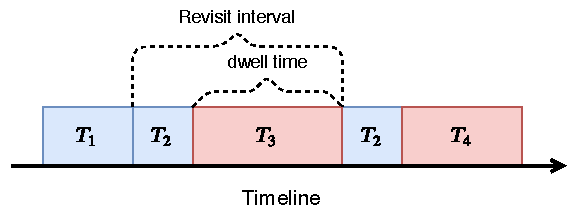
\includegraphics{big_picture.pdf}
    \caption{
        An example for tasks $T_i \forall i\in\{1,2,3,4\}$ that are scheduled on a radar timeline. 
        The revisit interval and dwell time is illustrated in the figure.
        The blue and red color illustrate different type of tasks such as tracking and search tasks.
        The task scheduler should generate the timeline such that cumulative reward function is maximized. 
    }
    \label{fig:big_picture}
\end{figure}

\subsection{Task-based time budget management}

\subsubsection{Multi-armed bandits for beam scheduling in multitarget tracking}

The TBM for multitarget tracking can modeled as a partially observable Markov decision process \cite{Krishnamurthy1999, Krishnamurthy2001, Scala2006}.
The large state space of the POMDP problem can be relaxed by assuming Markovian multi-armed bandit formulation,  in which the target states are modeled with hidden Markov models with known model dynamics \cite{Krishnamurthy1999, Krishnamurthy2001}.
In the multi-armed bandit formulation the target Markov state evolves only if it has been observed.
Such assumption is inappropriate since the targets can move even if they are not observed.
The restless multi-armed formulation enables each target state to evolve concurrently \cite{Scala2006}.
However, in general the optimal solution for the RMAB problem is NP-hard \cite{Guha2007}.
Performance of a myopic solution was investigated in \cite{Scala2006}.
The target which minimizes the sum of predicted uncertainties was chosen at each scheduling interval.
The myopic policy was claimed to be optimal in the assumed simple scenario with two targets.
However, the myopic policy is suboptimal in general setting where multiple targets could exist or when the environment dynamics are more complex.

\subsubsection{Information based beam scheduling} \label{sec:inf_based}

A myopic information theoretic approach for beam direction scheduling was proposed in \cite{Kastella1997}.
The surveillance area was divided into smaller grid cells.
It is possible to calculate the probability of target existing in a given grid cell based on prior probabilities and past observations. 
Moreover, the radar can decide which cells are observed by deciding the illumination direction.
The track and search tasks are joined such that observing different grids must minimize the uncertainty in the radar scenario.
Transition and birth probabilities for undetected targets need to be predefined for each cell when the information theoretic approach is used.

An efficient non-myopic information based method  for multitarget search and tracking was proposed in \cite{Kreucher2004}.
It used particle filtering to obtain the posterior probabilities.
Joint multitarget probability density was used to determine the probabilities of target being in the given cell.
An approximation was used to approximate the Bellman equation to account the long-term consequences. 
In \cite{Kreucher2005}, the approximate algorithm was compared to optimal non-myopic policy which was found by using Q-learning.
Different information theoretic measures for presenting the belief state was compared in \cite{Xu2010}.
Furthermore, a deep reinforcement learning algorithm was used to approximate the Bellman equation.

\subsubsection{Hierarchical time budget management}

Winterby \etal proposed a convenient framework for solving the TBM problem as a constrained Markov decision process \cite{Wintenby2006}.
They acknowledged the fact that solving the TBM problem with conventional POMDP methodology is computationally intractable.
Therefore, the TBM problem was decomposed into slow-time-scale (STS) and fast-time-scale (FTS) scheduling objectives.
The STS scheduler decides a batch of sensing tasks to be executed in the next time horizon.
The order of the tasks inside the batch is arranged by the FTS scheduler.
Moreover, it is assumed that the order of the tasks executed between the STS intervals is nonessential.
In \cite{Wintenby2006}, a sensing task is considered to be realized as an algorithm that generates sequence of sensing actions to achieve the goal of the task.
In target tracking, such algorithms can have for example repeated attempts to find a target in case of missing detections \cite{Wintenby2006}.
As a result, the sensing task execution times can be stochastic.
The TBM was considered in STS by formulating the Markov decision process as an optimization problem by using multiple different relaxations.


\subsubsection{Optimized dwell durations for target tracking and search}

Byrne proposed in \cite{Byrne2015, Byrne2016} an optimization approach for scheduling radar dwells to minimize a cost function. 
The cost function was designed to handle search and tracking functions separately.
In the approach, dwell durations for each radar task was optimized for the next scheduling interval, and constraints was applied to limit the sum of the dwell durations below the scheduling interval length.
First, a myopic cost function was optimized in \cite{Byrne2015}, and afterwards in \cite{Byrne2016} a non-myopic approach was proposed to optimize the long term costs.
The cost function was based on penalizing sensing actions that did not achieve track update or did not detect an undetected target.
Thus, costs for not detecting an undetected target in a surveillance area and not updating an existing track needed to be defined.
In addition, the cost function required defining a probability distributions for arriving new targets, and target transition probabilities between the cells for undetected targets.
The search space was discretized as in \cite{Kreucher2004} such that the arrival and transition probabilities for undetected targets can be defined.
The overall cost function is formed by weighting the search and tracking costs by the probability that such event happens and summing all the weighted costs together.
The cost function emphasizes taking sensing actions that balance well the overall search and tracking costs based on the assumed probability distributions.

\subsection{Adaptive revisit interval algorithms for time budget management} \label{sec:tbm_ri}

The radar time resources can be released from tracking tasks by decreasing the revisit interval. 
The interval should be adjusted such that it is possible to keep tracking the target and to minimize the tracking load.
Shorter revisit intervals should be used for maneuvering targets with higher process noise in order to keep state estimates on a tolerable level. 
Similarly, larger revisit interval should be used for non maneuvering targets with stationary trajectory because the movement is more predictable.
Different adaptive revisit interval algorithms have been widely studied to release time resources from target tracking to other radar tasks \cite{Cohen1986, Gardner1988, Munu1992, ChengTing2007, Baek2010, Watson1993, Charlish2015, Keuk1975, Shin1995, Benoudnine2006, Esfahani2012, Mofrad2017, Christiansen2018, Pilte2018}.
The algorithms are briefly covered in the following sections. 

\subsubsection{Residual based algorithms}

In \cite{Cohen1986}, Cohen \etal introduced a novel approach for adaptively choosing the revisit interval using a residual-based approach.
The residual between a measurement $y(k)$ and a prediction $x(k)$ was calculated as follows
\begin{equation}\label{eq:innovation}
    e(k) = y(k) - \hat{x}(k),
\end{equation}
and it is also called an innovation.
Furthermore, the innovation was normalized with measurement noise standard deviation $\sigma_m$ such that 
\begin{equation}\label{eq:norm_residual}
    e_n(k) = \frac{|e(k)|}{\sigma_m}.
\end{equation}
The revisit interval was increased or decreased by using simple recursive rule 
\begin{equation}\label{eq:update_resid}
    T(k) = \frac{T(k-1)}{\sqrt{e_n(k)}}.
\end{equation}
An $\alpha \beta$ filter was used and the revisit interval was controlled using the equations \eqref{eq:innovation},\eqref{eq:norm_residual} and \eqref{eq:update_resid}.
In \cite{Gardner1988} the work of Cohen was was extended for $\alpha\beta\gamma$ filters in which the cube root of the normalized residual \eqref{eq:norm_residual} was used in the equation \eqref{eq:update_resid}.
Moreover, it was suggested to smooth the large variations in $e(n)$ by using a first-order low-pass filter.
The performance between the $\alpha\beta$ and the $\alpha\beta\gamma$ filters were compared in \cite{Munu1992}.
It was found out that $\alpha\beta\gamma$ filters can execute with longer update intervals when the target is maneuvering.
Moreover, the cube root filter did achieve a better compromise between the tracking accuracy and the revisit interval.     
For constant velocity targets, the $\alpha\beta$ filter was more appropriate because it smooths the data better.

A residual-based algorithm for the IMM estimator was proposed in \cite{ChengTing2007}.
The following equation was obtained for calculating the revisit interval
\begin{equation}
    T(k) = \frac{4}{2^p}, \text{ } 4^p c < |e_s(k)| < 4^{p+1}c
\end{equation}
in which $e_s(n)$ is the normalized and smoothed residual.
Furthermore, equation for $p$ can be written as
\begin{equation}
    p = \floor*{\log_4\frac{1}{c}|e_s(k)|}
\end{equation}
where $c$ is variable that can be used to control trade-off between the accuracy and the tracking load.
Also, the maximum update interval was specified for the algorithm based on the used tracking models.

Baek \etal in \cite{Baek2010} proposed a residual-based algorithm in which the residual between the position measurement and the position estimate is wanted to keep below the desired threshold.
A simple recursive update rule was obtained
\begin{equation}
    T(k) = T(k - 1) \sqrt{\frac{e_0}{e(k)}},
\end{equation}
where $e_0$ is the desired maximum expected residual.

\subsubsection{Van Keuk's criterion}

Van Keuk proposed a criterion in \cite{Keuk1975} that can be utilized to calculate revisit interval efficiently.
Initially, the idea was considered one-dimensional space.
The revisit interval optimization problem was formulated as a solution for the following criterion
\begin{equation} \label{eq:criterion}
    \sigma_p^2(k + T | k) = V_0^2 \sigma_m^2
\end{equation}
where $\sigma_p^2(k + T | k)$ is the position prediction error variance, $\sigma_m^2$ is the measurement error variance, and
the parameter $V_0$ was called track sharpness.
The approach assumed a Singer target model with an acceleration standard deviation parameter $\Sigma$ and correlation parameter $\Theta$.
Using the assumed models and steady-state Kalman filter equations, a heuristic rule to calculate $T$ was obtained
\begin{equation}\label{eq:keuk_time}
    T \approx 0.4 \left[ \frac{\sigma_m \sqrt{\Theta}}{\Sigma} \right]^{0.4} \frac{V_0^{2.4}}{1+\frac{1}{2}V_0^2}
\end{equation}
which approximately fulfils the equation \eqref{eq:criterion}.
In higher dimensions, $\sigma_p^2(t + T | t)$ is the maximum eigenvalue of the predicted position error matrix, and $\sigma_m^2$ is the measurement error variance in the corresponding direction.

The efficient equation \eqref{eq:keuk_time} for calculating the revisit interval was found in \cite{Keuk1975} but the optimal value for the track sharpness parameter $V_0$ was not considered.
However, the work was extended in \cite{vanKeuk1993} to find suitable value for $V_0$ by considering the tracking load
\begin{equation}\label{eq:load}
    L = \frac{\E{n}}{T}
\end{equation}
where $n$ is the number of dwells needed to obtain the detection.
It was assumed that only angular uncertainty is needed to consider when \eqref{eq:load} was intended to minimize, 
because it enables pointing the beam in the correct direction.
Therefore, the criterion \eqref{eq:criterion} was modified by replacing the parameter $\sigma_m^2$ with the half-power beamwidth $B$ of the transmitted beam.
\begin{equation} \label{eq:criterion2}
    G(t + T | t) = V_0 B
\end{equation}
A refined version of the revisit interval rule was obtained based on the half-power beam width
\begin{equation}
    T \approx 0.4 \left[ \frac{\sigma_m r \sqrt{\Theta}}{\Sigma} \right]^{0.4} \frac{U^{2.4}}{1+\frac{1}{2}U^2}
\end{equation}
where $r$ is the distance from the radar to the target, and variance reduction parameter was defined as
\begin{equation}
    U = \frac{V_0 B}{\sigma_m}.
\end{equation}
Value for $V_0$ can be found by minimizing equation \eqref{eq:load} where $\E{n}$ and $T$ are substituted with their closed form equations.

The research in \cite{Keuk1975, vanKeuk1993} was based on finding the formula to calculate the revisit interval for the Singer model with known maneuver parameters.
However, in \cite{Shin1995} the work was extended for IMM estimators where the maneuver parameters can be easily calculated online.
In other words, the maneuver parameters $\Theta$ and $\Sigma$ was calculated from the used models and their posterior model probabilities.
All the other results from Keuk's work could be still utilized as before.

\subsubsection{Predicted error covariance based methods}

Novel work for optimizing the revisit interval to maintain desired state prediction error was carried out in \cite{Watson1993}.
The work was done for the IMM estimators for which the predicted error covariance matrix can be calculated by weighting the covariance matrices of the individual models with the model probabilities.
A threshold for the uncertainty was used which was proportional to the measurement error covariance matrix.
Furthermore, the threshold matrix and predicted covariance was set equal as follows  
\begin{equation}\label{eq:cov_th}
    \tr{ \vec{P}_{t+T|t} } = \tr{ \vec{P}_{\text{th}} }
\end{equation}
where $\vec{P}_{t+T|t}$ is the predicted error covariance, and $\vec{P}_{\text{th}}$ is the threshold covariance matrix.
From the equation \eqref{eq:cov_th}, a polynomial function was obtained which is function of the revisit interval $T$.
The non-linear optimization problem was optimized using Newton's method.

In \cite{Charlish2015} it is shown that it may be beneficial to introduce anticipation for the revisit interval algorithms.
The anticipation is utilized to prevent large prediction errors when the target moves through an occluded area by acquiring state prediction accuracy beforehand.
Mathematically the anticipation is acquired by maximizing the discounted long-term reward function.
In other words, the POMDP framework was utilized where the reward function was defined as
\begin{equation}
    R(b_t, T) = \frac{u\left(\vec{P}_{t+T|t} \right) T^2}{\tau_c}
\end{equation}
where $b_t$ is the belief state, and $\tau_c$ is the measurement duration.
The utility function $u\left(\vec{P}_{t+T|t} \right)=1$ if desired tracking accuracy is achieved.
Otherwise, tracking accuracy below the threshold gradually decreases the utility function towards zero.



\subsubsection{Other approaches}

\newcommand{\tmax}{T_\text{max}}
\newcommand{\tmin}{T_\text{min}}
\newcommand{\muca}{\mu_{\text{CA}}}
\newcommand{\mucv}{\mu_{\text{CV}}}

Benoudnine \etal proposed in \cite{Benoudnine2006} an IMM estimator with simplified architecture and a fast algorithm for calculating the revisit interval.
The IMM filter had two models, a constant velocity model, and a constant acceleration model.
The maximum revisit interval $\tmax$ was defined for the constant velocity model.
Similarly, the minimum revisit interval $\tmin$ was defined for the constant acceleration model.
The revisit interval was obtained with a simplified rule
\begin{equation}
    T = \muca \tmin + \mucv \tmax,
\end{equation}
where $\mucv$ and $\muca$ are the probabilities for constant velocity and constant acceleration models, respectively.

Masoumi-Ganjgah \etal proposed in \cite{Masoumi-Ganjgah2017} an algorithm which is closely related to algorithm proposed in \cite{Benoudnine2006}.
An IMM estimator with three different maneuver models was used, and parameters $\tmax$ and $\tmin$ were was defined for the models.
The models was designed to have different maneuvering levels starting from low maneuvering model to high maneuvering model.
Also, the revisit interval was adjusted different way as in \cite{Benoudnine2006}.
The revisit interval was controlled recursively such that if the highest maneuvering model had the highest posterior probability, then 
revisit interval was decreased with constant scalar less than $1$.
On the other hand, if the lowest maneuvering model with had the highest posterior probability, then
revisit interval was increased with constant scalar greater than $1$.
Otherwise, the revisit interval was kept the same as in the last interval.

Esfahani and Kamarei in \cite{Esfahani2012} proposed a non-myopic optimization method for solving the subset of tasks to be executed in the next scheduling interval.
The approach was closely related to the adaptive update interval methods and hierarchical TBM methods.
It could be interpreted that the paper extends the adaptive update interval algorithms for multiple targets.
An algorithm was developed to find a subset of targets to be updated in the next scheduling using the optimal interval such that target localization accuracy is maximized.
Consequently, the search task of the multifunction radar was not included in the formulation.
The approach is stated to be non-myopic since it does not try to maximize the instantaneous cost function.
However, the method does not fully take into account the long-term consequences when planning the scheduling intervals.
The tasks that have the closest deadlines are scheduled for the current scheduling interval.

\begin{itemize}
    \item \cite{Christiansen2018} Uses fisher information criteria etc. to calculate the update interval
    \item \cite{Pilte2018} Derives adaptive update rate for non-linear trackers
\end{itemize}

\newpage
\section{Reinforcement learning approach for revisit interval selection}

The existing research in adaptive revisit interval algorithms was reviewed in section \ref{sec:tbm_ri}.
It was identified that existing algorithms control the revisit interval based on the innovation or the uncertainty on the estimates.
The residual based methods are less dependent on the system model since the average residuals are kept near the noise standard deviation using a recursive rule \eqref{eq:update_resid}.
The covariance matrix based algorithms are less robust for model inaccuracies because the dynamic model is used to calculate the intervals.
However, the latter approach is more transparent since the covariance estimates are kept below a certain threshold.

The performance of an adaptive revisit interval algorithm is usually quantified by the achieved accuracy in the state estimates.
Especially, the position estimate is important for pointing the radar beam in the correct direction.
However, the purpose of applying adaptive revisit interval algorithms is to minimize the time allocation of the tracking task.
The time allocation can be quantified with the track load which is the relation between the dwell duration and the revisit interval \cite{vanKeuk1993}.

A commonly used tracking filter is an IMM filter that can be used to track targets with various maneuvers.
The filter consists of multiple Kalman filters which are configured for different maneuvers.
All the Kalman filters are concurrently used to track the targets.
The probability of a measurement coming from a given Kalman filter state-space model can be extracted for each filter.
The probabilities can be used to calculate estimates on the process noise and the kinematic state.

Here a reinforcement learning approach is proposed for controlling the revisit interval of the tracking filter.
The reinforcement learning agent is capable of learning directly from the experience such that 
environment model is not needed to optimize the employed reward function.
Moreover, the approach applies to any tracking filter.
The motivation for using reinforcement learning is to learn near-optimal policy which can adapt to any tracking system, enables including the anticipation which was described in \cite{Charlish2015}, and enables using observation data with non-trivial connection to the revisit interval.

\subsection{Actions}

The agent is controlling the revisit interval of the tracking filter.
It is assumed that each track update consists of searching the target as long as the target is detected or
when a certain upper limit is reached.
A discretized set of different time intervals is used.

\subsection{Reward}

Time is one of the most valuable assets for the multifunction radar.
A reward function that minimizes the tracking load and encourages to keep desired tracking accuracy is used.
The reward function is defined as in \cite{Charlish2015}
\begin{equation}
    r_t = \frac{u(P_t) T}{\tau}
\end{equation}
where $\tau$ is the dwell length, $u(P_t) \in (0, 1)$ is tracking accuracy function, $P_t$ is the posterior estimate of the  state error covariance matrix, and $T$ is the revisit interval.
The tracking accuracy function is $1$ if the accuracy is better than the threshold for the covariance matrix.
Otherwise, $u(P) < 1$ if accuracy is worse than the threshold.
Different from \cite{Charlish2015}, the dwell length $d$ is considered to be function of SINR and position uncertainty \cite{vanKeuk1993}.
The reward definition enables the agent to trade-off the accuracy for the scenarios where the load is more important.
For example, in overload situations, the agent should prefer to use revisit intervals which minimize the load.


\subsection{States and observations}

The target movement can be modeled as a jump linear Markov system (JLMS).
In JMLS, the movement is described by a linear state-space model, and the linear state-space model has different parameterizations.
The transitions between the parameterizations are described with the Markov chain.
The state of the target is partially observable thus it is a hidden Markov model.
A state estimation algorithm such as the IMM algorithm can be used to extract the state from the noisy measurements.
The performance of the tracking algorithm is based on the model accuracy.

The environment state for the reinforcement learning agent is related to the tracking filter because the revisit interval is controlled based on the tracking filter performance.
The state of the tracking filter is described by how accurate the current estimates are, and what filter models are used to extract the observations.
For example, if the tracking filter currently relies on non-maneuvering models and the last couple residuals have been large, then the agent should decrease the revisit interval quite a lot to ensure that the filter state is changed to suitable maneuvering model. 
It may be noted that neither of the observations holds Markov's property since the extracted information contains noise.
Thus, reinforcement learning methods with memory should be used.
For example, neural networks with long short-term memory (LSTM).
Another approach is to use filtering to extract the average using the discounted sum as in \cite{Munu1992}.

\newpage
\section{Simulations}

A single target tracking scenario is considered in these simulations.
Different aspects that should be considered are
\begin{itemize}
    \item target trajectory generation,
    \item measurement model,
    \item design of the tracking algorithm, and
    \item implementation of the existing adaptive revisit interval algorithms.
\end{itemize}

\subsection{Target trajectory generation}

Target trajectory can be generated couple different ways.
The target state evolution could be generated though discrete-time linear stochastic equation \cite{Bar-Shalom2001}
\begin{equation}
    x_{t+1} = F_t x_t + B_t u_t + v_t
\end{equation}
with matrices $F_t$, $B_t$ and process noise $v_t \sim N(O, Q_t)$, where $Q_t$ is the process noise covariance matrix.
The model is convenient combine with Kalman filters because then optimal filtering can be applied.
However, using such a model can get quite complicated when the goal is to create realistic trajectories \cite{RongLi2003}.

Another approach for creating the trajectory is to use waypoint generator.
A batch of waypoints is given for the generator and the generator generates smooth trajectory based on them.
Furthermore, the trajectory points can be preprocessed to include noise.
This method can generate quite realistic trajectories, but designing a tracking filter for the trajectory is more complicated.

\subsection{Measurement model}

The 
The radar is used to track the hidden 

\subsection{Design of the tracking algorithm}

\newpage
\section{Conclusions}



\newpage
\bibliographystyle{IEEEtran}
\bibliography{references}


\end{document}
